\documentclass[11pt,compress,t,notes=noshow, xcolor=table]{beamer}
\usepackage[]{graphicx}\usepackage[]{color}
% maxwidth is the original width if it is less than linewidth
% otherwise use linewidth (to make sure the graphics do not exceed the margin)
\makeatletter
\def\maxwidth{ %
  \ifdim\Gin@nat@width>\linewidth
    \linewidth
  \else
    \Gin@nat@width
  \fi
}
\makeatother

\definecolor{fgcolor}{rgb}{0.345, 0.345, 0.345}
\newcommand{\hlnum}[1]{\textcolor[rgb]{0.686,0.059,0.569}{#1}}%
\newcommand{\hlstr}[1]{\textcolor[rgb]{0.192,0.494,0.8}{#1}}%
\newcommand{\hlcom}[1]{\textcolor[rgb]{0.678,0.584,0.686}{\textit{#1}}}%
\newcommand{\hlopt}[1]{\textcolor[rgb]{0,0,0}{#1}}%
\newcommand{\hlstd}[1]{\textcolor[rgb]{0.345,0.345,0.345}{#1}}%
\newcommand{\hlkwa}[1]{\textcolor[rgb]{0.161,0.373,0.58}{\textbf{#1}}}%
\newcommand{\hlkwb}[1]{\textcolor[rgb]{0.69,0.353,0.396}{#1}}%
\newcommand{\hlkwc}[1]{\textcolor[rgb]{0.333,0.667,0.333}{#1}}%
\newcommand{\hlkwd}[1]{\textcolor[rgb]{0.737,0.353,0.396}{\textbf{#1}}}%
\let\hlipl\hlkwb

\usepackage{framed}
\makeatletter
\newenvironment{kframe}{%
 \def\at@end@of@kframe{}%
 \ifinner\ifhmode%
  \def\at@end@of@kframe{\end{minipage}}%
  \begin{minipage}{\columnwidth}%
 \fi\fi%
 \def\FrameCommand##1{\hskip\@totalleftmargin \hskip-\fboxsep
 \colorbox{shadecolor}{##1}\hskip-\fboxsep
     % There is no \\@totalrightmargin, so:
     \hskip-\linewidth \hskip-\@totalleftmargin \hskip\columnwidth}%
 \MakeFramed {\advance\hsize-\width
   \@totalleftmargin\z@ \linewidth\hsize
   \@setminipage}}%
 {\par\unskip\endMakeFramed%
 \at@end@of@kframe}
\makeatother

\definecolor{shadecolor}{rgb}{.97, .97, .97}
\definecolor{messagecolor}{rgb}{0, 0, 0}
\definecolor{warningcolor}{rgb}{1, 0, 1}
\definecolor{errorcolor}{rgb}{1, 0, 0}
\newenvironment{knitrout}{}{} % an empty environment to be redefined in TeX

\usepackage{alltt}
\newcommand{\SweaveOpts}[1]{}  % do not interfere with LaTeX
\newcommand{\SweaveInput}[1]{} % because they are not real TeX commands
\newcommand{\Sexpr}[1]{}       % will only be parsed by R
\newcommand{\xmark}{\ding{55}}%


\usepackage[english]{babel}
\usepackage[utf8]{inputenc}

\usepackage{dsfont}
\usepackage{verbatim}
\usepackage{amsmath}
\usepackage{amsfonts}
\usepackage{amssymb}
\usepackage{bm}
\usepackage{csquotes}
\usepackage{multirow}
\usepackage{longtable}
\usepackage{booktabs}
\usepackage{enumerate}
\usepackage[absolute,overlay]{textpos}
\usepackage{psfrag}
\usepackage{algorithm}
\usepackage{algpseudocode}
\usepackage{eqnarray}
\usepackage{arydshln}
\usepackage{tabularx}
\usepackage{placeins}
\usepackage{tikz}
\usepackage{setspace}
\usepackage{colortbl}
\usepackage{mathtools}
\usepackage{wrapfig}
\usepackage{bm}
\usepackage{amsmath}
\usepackage{pifont}

\usetikzlibrary{shapes,arrows,automata,positioning,calc,chains,trees, shadows}
\tikzset{
  %Define standard arrow tip
  >=stealth',
  %Define style for boxes
  punkt/.style={
    rectangle,
    rounded corners,
    draw=black, very thick,
    text width=6.5em,
    minimum height=2em,
    text centered},
  % Define arrow style
  pil/.style={
    ->,
    thick,
    shorten <=2pt,
    shorten >=2pt,}
}

\usepackage{subfig}

% Defines macros and environments
\usepackage{../../style/lmu-lecture}


\let\code=\texttt
\let\proglang=\textsf

\setkeys{Gin}{width=0.9\textwidth}

\setbeamertemplate{frametitle}{\expandafter\uppercase\expandafter\insertframetitle}

\usepackage{bbm}
% basic latex stuff
\newcommand{\pkg}[1]{{\fontseries{b}\selectfont #1}} %fontstyle for R packages
\newcommand{\lz}{\vspace{0.5cm}} %vertical space
\newcommand{\dlz}{\vspace{1cm}} %double vertical space
\newcommand{\oneliner}[1] % Oneliner for important statements
{\begin{block}{}\begin{center}\begin{Large}#1\end{Large}\end{center}\end{block}}


%new environments
\newenvironment{vbframe}  %frame with breaks and verbatim
{
 \begin{frame}[containsverbatim,allowframebreaks]
}
{
\end{frame}
}

\newenvironment{vframe}  %frame with verbatim without breaks (to avoid numbering one slided frames)
{
 \begin{frame}[containsverbatim]
}
{
\end{frame}
}

\newenvironment{blocki}[1]   % itemize block
{
 \begin{block}{#1}\begin{itemize}
}
{
\end{itemize}\end{block}
}

\newenvironment{fragileframe}[2]{  %fragile frame with framebreaks
\begin{frame}[allowframebreaks, fragile, environment = fragileframe]
\frametitle{#1}
#2}
{\end{frame}}


\newcommand{\myframe}[2]{  %short for frame with framebreaks
\begin{frame}[allowframebreaks]
\frametitle{#1}
#2
\end{frame}}

\newcommand{\remark}[1]{
  \textbf{Remark:} #1
}

\newcommand{\citebutton}[2]{%
\NoCaseChange{\resizebox{!}{9pt}{\protect\beamergotobutton{\href{#2}{#1}}}}%
}



\newenvironment{deleteframe}
{
\begingroup
\usebackgroundtemplate{\includegraphics[width=\paperwidth,height=\paperheight]{../style/color/red.png}}
 \begin{frame}
}
{
\end{frame}
\endgroup
}
\newenvironment{simplifyframe}
{
\begingroup
\usebackgroundtemplate{\includegraphics[width=\paperwidth,height=\paperheight]{../style/color/yellow.png}}
 \begin{frame}
}
{
\end{frame}
\endgroup
}\newenvironment{draftframe}
{
\begingroup
\usebackgroundtemplate{\includegraphics[width=\paperwidth,height=\paperheight]{../style/color/green.jpg}}
 \begin{frame}
}
{
\end{frame}
\endgroup
}
% https://tex.stackexchange.com/a/261480: textcolor that works in mathmode
\makeatletter
\renewcommand*{\@textcolor}[3]{%
  \protect\leavevmode
  \begingroup
    \color#1{#2}#3%
  \endgroup
}
\makeatother





% math spaces
\ifdefined\N                                                                
\renewcommand{\N}{\mathds{N}} % N, naturals
\else \newcommand{\N}{\mathds{N}} \fi 
\newcommand{\Z}{\mathds{Z}} % Z, integers
\newcommand{\Q}{\mathds{Q}} % Q, rationals
\newcommand{\R}{\mathds{R}} % R, reals
\ifdefined\C 
  \renewcommand{\C}{\mathds{C}} % C, complex
\else \newcommand{\C}{\mathds{C}} \fi
\newcommand{\continuous}{\mathcal{C}} % C, space of continuous functions
\newcommand{\M}{\mathcal{M}} % machine numbers
\newcommand{\epsm}{\epsilon_m} % maximum error

% counting / finite sets
\newcommand{\setzo}{\{0, 1\}} % set 0, 1
\newcommand{\setmp}{\{-1, +1\}} % set -1, 1
\newcommand{\unitint}{[0, 1]} % unit interval

% basic math stuff
\newcommand{\xt}{\tilde x} % x tilde
\newcommand{\argmax}{\operatorname{arg\,max}} % argmax
\newcommand{\argmin}{\operatorname{arg\,min}} % argmin
\newcommand{\argminlim}{\mathop{\mathrm{arg\,min}}\limits} % argmax with limits
\newcommand{\argmaxlim}{\mathop{\mathrm{arg\,max}}\limits} % argmin with limits  
\newcommand{\sign}{\operatorname{sign}} % sign, signum
\newcommand{\I}{\mathbb{I}} % I, indicator
\newcommand{\order}{\mathcal{O}} % O, order
\newcommand{\pd}[2]{\frac{\partial{#1}}{\partial #2}} % partial derivative
\newcommand{\floorlr}[1]{\left\lfloor #1 \right\rfloor} % floor
\newcommand{\ceillr}[1]{\left\lceil #1 \right\rceil} % ceiling

% sums and products
\newcommand{\sumin}{\sum\limits_{i=1}^n} % summation from i=1 to n
\newcommand{\sumim}{\sum\limits_{i=1}^m} % summation from i=1 to m
\newcommand{\sumjn}{\sum\limits_{j=1}^n} % summation from j=1 to p
\newcommand{\sumjp}{\sum\limits_{j=1}^p} % summation from j=1 to p
\newcommand{\sumik}{\sum\limits_{i=1}^k} % summation from i=1 to k
\newcommand{\sumkg}{\sum\limits_{k=1}^g} % summation from k=1 to g
\newcommand{\sumjg}{\sum\limits_{j=1}^g} % summation from j=1 to g
\newcommand{\meanin}{\frac{1}{n} \sum\limits_{i=1}^n} % mean from i=1 to n
\newcommand{\meanim}{\frac{1}{m} \sum\limits_{i=1}^m} % mean from i=1 to n
\newcommand{\meankg}{\frac{1}{g} \sum\limits_{k=1}^g} % mean from k=1 to g
\newcommand{\prodin}{\prod\limits_{i=1}^n} % product from i=1 to n
\newcommand{\prodkg}{\prod\limits_{k=1}^g} % product from k=1 to g
\newcommand{\prodjp}{\prod\limits_{j=1}^p} % product from j=1 to p

% linear algebra
\newcommand{\one}{\boldsymbol{1}} % 1, unitvector
\newcommand{\zero}{\mathbf{0}} % 0-vector
\newcommand{\id}{\boldsymbol{I}} % I, identity
\newcommand{\diag}{\operatorname{diag}} % diag, diagonal
\newcommand{\trace}{\operatorname{tr}} % tr, trace
\newcommand{\spn}{\operatorname{span}} % span
\newcommand{\scp}[2]{\left\langle #1, #2 \right\rangle} % <.,.>, scalarproduct
\newcommand{\mat}[1]{\begin{pmatrix} #1 \end{pmatrix}} % short pmatrix command
\newcommand{\Amat}{\mathbf{A}} % matrix A
\newcommand{\Deltab}{\mathbf{\Delta}} % error term for vectors

% basic probability + stats
\renewcommand{\P}{\mathds{P}} % P, probability
\newcommand{\E}{\mathds{E}} % E, expectation
\newcommand{\var}{\mathsf{Var}} % Var, variance
\newcommand{\cov}{\mathsf{Cov}} % Cov, covariance
\newcommand{\corr}{\mathsf{Corr}} % Corr, correlation
\newcommand{\normal}{\mathcal{N}} % N of the normal distribution
\newcommand{\iid}{\overset{i.i.d}{\sim}} % dist with i.i.d superscript
\newcommand{\distas}[1]{\overset{#1}{\sim}} % ... is distributed as ...

% machine learning
\newcommand{\Xspace}{\mathcal{X}} % X, input space
\newcommand{\Yspace}{\mathcal{Y}} % Y, output space
\newcommand{\nset}{\{1, \ldots, n\}} % set from 1 to n
\newcommand{\pset}{\{1, \ldots, p\}} % set from 1 to p
\newcommand{\gset}{\{1, \ldots, g\}} % set from 1 to g
\newcommand{\Pxy}{\mathbb{P}_{xy}} % P_xy
\newcommand{\Exy}{\mathbb{E}_{xy}} % E_xy: Expectation over random variables xy
\newcommand{\xv}{\mathbf{x}} % vector x (bold)
\newcommand{\xtil}{\tilde{\mathbf{x}}} % vector x-tilde (bold)
\newcommand{\yv}{\mathbf{y}} % vector y (bold)
\newcommand{\xy}{(\xv, y)} % observation (x, y)
\newcommand{\xvec}{\left(x_1, \ldots, x_p\right)^\top} % (x1, ..., xp) 
\newcommand{\Xmat}{\mathbf{X}} % Design matrix
\newcommand{\allDatasets}{\mathds{D}} % The set of all datasets
\newcommand{\allDatasetsn}{\mathds{D}_n}  % The set of all datasets of size n 
\newcommand{\D}{\mathcal{D}} % D, data
\newcommand{\Dn}{\D_n} % D_n, data of size n
\newcommand{\Dtrain}{\mathcal{D}_{\text{train}}} % D_train, training set
\newcommand{\Dtest}{\mathcal{D}_{\text{test}}} % D_test, test set
\newcommand{\xyi}[1][i]{\left(\xv^{(#1)}, y^{(#1)}\right)} % (x^i, y^i), i-th observation
\newcommand{\Dset}{\left( \xyi[1], \ldots, \xyi[n]\right)} % {(x1,y1)), ..., (xn,yn)}, data
\newcommand{\defAllDatasetsn}{(\Xspace \times \Yspace)^n} % Def. of the set of all datasets of size n 
\newcommand{\defAllDatasets}{\bigcup_{n \in \N}(\Xspace \times \Yspace)^n} % Def. of the set of all datasets 
\newcommand{\xdat}{\left\{ \xv^{(1)}, \ldots, \xv^{(n)}\right\}} % {x1, ..., xn}, input data
\newcommand{\yvec}{\left(y^{(1)}, \hdots, y^{(n)}\right)^\top} % (y1, ..., yn), vector of outcomes
\renewcommand{\xi}[1][i]{\xv^{(#1)}} % x^i, i-th observed value of x
\newcommand{\yi}[1][i]{y^{(#1)}} % y^i, i-th observed value of y 
\newcommand{\xivec}{\left(x^{(i)}_1, \ldots, x^{(i)}_p\right)^\top} % (x1^i, ..., xp^i), i-th observation vector
\newcommand{\xj}{\xv_j} % x_j, j-th feature
\newcommand{\xjvec}{\left(x^{(1)}_j, \ldots, x^{(n)}_j\right)^\top} % (x^1_j, ..., x^n_j), j-th feature vector
\newcommand{\phiv}{\mathbf{\phi}} % Basis transformation function phi
\newcommand{\phixi}{\mathbf{\phi}^{(i)}} % Basis transformation of xi: phi^i := phi(xi)

%%%%%% ml - models general
\newcommand{\lamv}{\bm{\lambda}} % lambda vector, hyperconfiguration vector
\newcommand{\Lam}{\bm{\Lambda}}	 % Lambda, space of all hpos
% Inducer / Inducing algorithm
\newcommand{\preimageInducer}{\left(\defAllDatasets\right)\times\Lam} % Set of all datasets times the hyperparameter space
\newcommand{\preimageInducerShort}{\allDatasets\times\Lam} % Set of all datasets times the hyperparameter space
% Inducer / Inducing algorithm
\newcommand{\ind}{\mathcal{I}} % Inducer, inducing algorithm, learning algorithm 

% continuous prediction function f
\newcommand{\ftrue}{f_{\text{true}}}  % True underlying function (if a statistical model is assumed)
\newcommand{\ftruex}{\ftrue(\xv)} % True underlying function (if a statistical model is assumed)
\newcommand{\fx}{f(\xv)} % f(x), continuous prediction function
\newcommand{\fdomains}{f: \Xspace \rightarrow \R^g} % f with domain and co-domain
\newcommand{\Hspace}{\mathcal{H}} % hypothesis space where f is from
\newcommand{\fbayes}{f^{\ast}} % Bayes-optimal model
\newcommand{\fxbayes}{f^{\ast}(\xv)} % Bayes-optimal model
\newcommand{\fkx}[1][k]{f_{#1}(\xv)} % f_j(x), discriminant component function
\newcommand{\fh}{\hat{f}} % f hat, estimated prediction function
\newcommand{\fxh}{\fh(\xv)} % fhat(x)
\newcommand{\fxt}{f(\xv ~|~ \thetab)} % f(x | theta)
\newcommand{\fxi}{f\left(\xv^{(i)}\right)} % f(x^(i))
\newcommand{\fxih}{\hat{f}\left(\xv^{(i)}\right)} % f(x^(i))
\newcommand{\fxit}{f\left(\xv^{(i)} ~|~ \thetab\right)} % f(x^(i) | theta)
\newcommand{\fhD}{\fh_{\D}} % fhat_D, estimate of f based on D
\newcommand{\fhDtrain}{\fh_{\Dtrain}} % fhat_Dtrain, estimate of f based on D
\newcommand{\fhDnlam}{\fh_{\Dn, \lamv}} %model learned on Dn with hp lambda
\newcommand{\fhDlam}{\fh_{\D, \lamv}} %model learned on D with hp lambda
\newcommand{\fhDnlams}{\fh_{\Dn, \lamv^\ast}} %model learned on Dn with optimal hp lambda 
\newcommand{\fhDlams}{\fh_{\D, \lamv^\ast}} %model learned on D with optimal hp lambda 

% discrete prediction function h
\newcommand{\hx}{h(\xv)} % h(x), discrete prediction function
\newcommand{\hh}{\hat{h}} % h hat
\newcommand{\hxh}{\hat{h}(\xv)} % hhat(x)
\newcommand{\hxt}{h(\xv | \thetab)} % h(x | theta)
\newcommand{\hxi}{h\left(\xi\right)} % h(x^(i))
\newcommand{\hxit}{h\left(\xi ~|~ \thetab\right)} % h(x^(i) | theta)
\newcommand{\hbayes}{h^{\ast}} % Bayes-optimal classification model
\newcommand{\hxbayes}{h^{\ast}(\xv)} % Bayes-optimal classification model

% yhat
\newcommand{\yh}{\hat{y}} % yhat for prediction of target
\newcommand{\yih}{\hat{y}^{(i)}} % yhat^(i) for prediction of ith targiet
\newcommand{\resi}{\yi- \yih}

% theta
\newcommand{\thetah}{\hat{\theta}} % theta hat
\newcommand{\thetab}{\bm{\theta}} % theta vector
\newcommand{\thetabh}{\bm{\hat\theta}} % theta vector hat
\newcommand{\thetat}[1][t]{\thetab^{[#1]}} % theta^[t] in optimization
\newcommand{\thetatn}[1][t]{\thetab^{[#1 +1]}} % theta^[t+1] in optimization
\newcommand{\thetahDnlam}{\thetabh_{\Dn, \lamv}} %theta learned on Dn with hp lambda
\newcommand{\thetahDlam}{\thetabh_{\D, \lamv}} %theta learned on D with hp lambda
\newcommand{\mint}{\min_{\thetab \in \Theta}} % min problem theta
\newcommand{\argmint}{\argmin_{\thetab \in \Theta}} % argmin theta

% densities + probabilities
% pdf of x 
\newcommand{\pdf}{p} % p
\newcommand{\pdfx}{p(\xv)} % p(x)
\newcommand{\pixt}{\pi(\xv~|~ \thetab)} % pi(x|theta), pdf of x given theta
\newcommand{\pixit}{\pi\left(\xi ~|~ \thetab\right)} % pi(x^i|theta), pdf of x given theta
\newcommand{\pixii}{\pi\left(\xi\right)} % pi(x^i), pdf of i-th x 

% pdf of (x, y)
\newcommand{\pdfxy}{p(\xv,y)} % p(x, y)
\newcommand{\pdfxyt}{p(\xv, y ~|~ \thetab)} % p(x, y | theta)
\newcommand{\pdfxyit}{p\left(\xi, \yi ~|~ \thetab\right)} % p(x^(i), y^(i) | theta)

% pdf of x given y
\newcommand{\pdfxyk}[1][k]{p(\xv | y= #1)} % p(x | y = k)
\newcommand{\lpdfxyk}[1][k]{\log p(\xv | y= #1)} % log p(x | y = k)
\newcommand{\pdfxiyk}[1][k]{p\left(\xi | y= #1 \right)} % p(x^i | y = k)

% prior probabilities
\newcommand{\pik}[1][k]{\pi_{#1}} % pi_k, prior
\newcommand{\lpik}[1][k]{\log \pi_{#1}} % log pi_k, log of the prior
\newcommand{\pit}{\pi(\thetab)} % Prior probability of parameter theta

% posterior probabilities
\newcommand{\post}{\P(y = 1 ~|~ \xv)} % P(y = 1 | x), post. prob for y=1
\newcommand{\postk}[1][k]{\P(y = #1 ~|~ \xv)} % P(y = k | y), post. prob for y=k
\newcommand{\pidomains}{\pi: \Xspace \rightarrow \unitint} % pi with domain and co-domain
\newcommand{\pibayes}{\pi^{\ast}} % Bayes-optimal classification model
\newcommand{\pixbayes}{\pi^{\ast}(\xv)} % Bayes-optimal classification model
\newcommand{\pix}{\pi(\xv)} % pi(x), P(y = 1 | x)
\newcommand{\pikx}[1][k]{\pi_{#1}(\xv)} % pi_k(x), P(y = k | x)
\newcommand{\pikxt}[1][k]{\pi_{#1}(\xv ~|~ \thetab)} % pi_k(x | theta), P(y = k | x, theta)
\newcommand{\pixh}{\hat \pi(\xv)} % pi(x) hat, P(y = 1 | x) hat
\newcommand{\pikxh}[1][k]{\hat \pi_{#1}(\xv)} % pi_k(x) hat, P(y = k | x) hat
\newcommand{\pixih}{\hat \pi(\xi)} % pi(x^(i)) with hat
\newcommand{\pikxih}[1][k]{\hat \pi_{#1}(\xi)} % pi_k(x^(i)) with hat
\newcommand{\pdfygxt}{p(y ~|~\xv, \thetab)} % p(y | x, theta)
\newcommand{\pdfyigxit}{p\left(\yi ~|~\xi, \thetab\right)} % p(y^i |x^i, theta)
\newcommand{\lpdfygxt}{\log \pdfygxt } % log p(y | x, theta)
\newcommand{\lpdfyigxit}{\log \pdfyigxit} % log p(y^i |x^i, theta)

% probababilistic
\newcommand{\bayesrulek}[1][k]{\frac{\P(\xv | y= #1) \P(y= #1)}{\P(\xv)}} % Bayes rule
\newcommand{\muk}{\bm{\mu_k}} % mean vector of class-k Gaussian (discr analysis) 

% residual and margin
\newcommand{\eps}{\epsilon} % residual, stochastic
\newcommand{\epsi}{\epsilon^{(i)}} % epsilon^i, residual, stochastic
\newcommand{\epsh}{\hat{\epsilon}} % residual, estimated
\newcommand{\yf}{y \fx} % y f(x), margin
\newcommand{\yfi}{\yi \fxi} % y^i f(x^i), margin
\newcommand{\Sigmah}{\hat \Sigma} % estimated covariance matrix
\newcommand{\Sigmahj}{\hat \Sigma_j} % estimated covariance matrix for the j-th class

% ml - loss, risk, likelihood
\newcommand{\Lyf}{L\left(y, f\right)} % L(y, f), loss function
\newcommand{\Lxy}{L\left(y, \fx\right)} % L(y, f(x)), loss function
\newcommand{\Lxyi}{L\left(\yi, \fxi\right)} % loss of observation
\newcommand{\Lxyt}{L\left(y, \fxt\right)} % loss with f parameterized
\newcommand{\Lxyit}{L\left(\yi, \fxit\right)} % loss of observation with f parameterized
\newcommand{\Lxym}{L\left(\yi, f\left(\bm{\tilde{x}}^{(i)} ~|~ \thetab\right)\right)} % loss of observation with f parameterized
\newcommand{\Lpixy}{L\left(y, \pix\right)} % loss in classification
\newcommand{\Lpixyi}{L\left(\yi, \pixii\right)} % loss of observation in classification
\newcommand{\Lpixyt}{L\left(y, \pixt\right)} % loss with pi parameterized
\newcommand{\Lpixyit}{L\left(\yi, \pixit\right)} % loss of observation with pi parameterized
\newcommand{\Lhxy}{L\left(y, \hx\right)} % L(y, h(x)), loss function on discrete classes
\newcommand{\Lr}{L\left(r\right)} % L(r), loss defined on residual (reg) / margin (classif)
\newcommand{\lone}{|y - \fx|} % L1 loss
\newcommand{\ltwo}{\left(y - \fx\right)^2} % L2 loss
\newcommand{\lbernoullimp}{\ln(1 + \exp(-y \cdot \fx))} % Bernoulli loss for -1, +1 encoding
\newcommand{\lbernoullizo}{- y \cdot \fx + \log(1 + \exp(\fx))} % Bernoulli loss for 0, 1 encoding
\newcommand{\lcrossent}{- y \log \left(\pix\right) - (1 - y) \log \left(1 - \pix\right)} % cross-entropy loss
\newcommand{\lbrier}{\left(\pix - y \right)^2} % Brier score
\newcommand{\risk}{\mathcal{R}} % R, risk
\newcommand{\riskbayes}{\mathcal{R}^\ast}
\newcommand{\riskf}{\risk(f)} % R(f), risk
\newcommand{\riskdef}{\E_{y|\xv}\left(\Lxy \right)} % risk def (expected loss)
\newcommand{\riskt}{\mathcal{R}(\thetab)} % R(theta), risk
\newcommand{\riske}{\mathcal{R}_{\text{emp}}} % R_emp, empirical risk w/o factor 1 / n
\newcommand{\riskeb}{\bar{\mathcal{R}}_{\text{emp}}} % R_emp, empirical risk w/ factor 1 / n
\newcommand{\riskef}{\riske(f)} % R_emp(f)
\newcommand{\risket}{\mathcal{R}_{\text{emp}}(\thetab)} % R_emp(theta)
\newcommand{\riskr}{\mathcal{R}_{\text{reg}}} % R_reg, regularized risk
\newcommand{\riskrt}{\mathcal{R}_{\text{reg}}(\thetab)} % R_reg(theta)
\newcommand{\riskrf}{\riskr(f)} % R_reg(f)
\newcommand{\riskrth}{\hat{\mathcal{R}}_{\text{reg}}(\thetab)} % hat R_reg(theta)
\newcommand{\risketh}{\hat{\mathcal{R}}_{\text{emp}}(\thetab)} % hat R_emp(theta)
\newcommand{\LL}{\mathcal{L}} % L, likelihood
\newcommand{\LLt}{\mathcal{L}(\thetab)} % L(theta), likelihood
\newcommand{\LLtx}{\mathcal{L}(\thetab | \xv)} % L(theta|x), likelihood
\newcommand{\logl}{\ell} % l, log-likelihood
\newcommand{\loglt}{\logl(\thetab)} % l(theta), log-likelihood
\newcommand{\logltx}{\logl(\thetab | \xv)} % l(theta|x), log-likelihood
\newcommand{\errtrain}{\text{err}_{\text{train}}} % training error
\newcommand{\errtest}{\text{err}_{\text{test}}} % test error
\newcommand{\errexp}{\overline{\text{err}_{\text{test}}}} % avg training error

% lm
\newcommand{\thx}{\thetab^\top \xv} % linear model
\newcommand{\olsest}{(\Xmat^\top \Xmat)^{-1} \Xmat^\top \yv} % OLS estimator in LM 


\newcommand{\titlefigure}{figure_man/ml_abstraction-crop.pdf}
\newcommand{\learninggoals}{
  \item \textcolor{blue}{XXX}
  \item \textcolor{blue}{XXX}
}

\title{Introduction to Machine Learning}
\date{}

\begin{document}

\lecturechapter{Advanced Performance Evaluation}
\lecture{Introduction to Machine Learning}
%
% \begin{vbframe}{Introduction}
% In predictive modeling, performance estimation can have different goals:
%
% \begin{itemize}
%   \item \textbf{Performance estimation of a model:}
%     Estimate \emph{generalization} error of a model on new (unseen) data, drawn from the same data generating process.
%   \item \textbf{Performance estimation of an algorithm:}
%     Estimate \emph{generalization} error of a learning algorithm, trained on a data set
%     of a certain size, on new (unseen) data, all drawn from the same data generating process.
%   \item \textbf{Model selection:}
%     Select the best model from a set of potential candidate models (e.g., different model classes, different
%     hyperparameter settings, different feature sets)
%   \item \textbf{Learning curves}
%     How does the generalization error scale when an algorithm is trained on training sets of different sizes?
% \end{itemize}
%
% Obviously, these goals are closely related: achieving reliable estimates of (predictive) performance
%
% \end{vbframe}

\begin{vbframe}{Generalization error of a model}

The \textbf{generalization error of a model} (also known as \textbf{model performance}) is defined as the expected loss of a fixed model $\fhD$ over $\Pxy$:

$$
GE\left(\fhD\right) = \E_{\xy \sim \Pxy}\left( L(y, \fhD(\xv))\right),
$$

where

\begin{itemize}
\item $\D$ is a dataset of size $n$ drawn from the joint $\Pxy$.
\item $\fhD = \mathcal{I}_{L, O}(\D)$ is a model induced by applying learning algorithm $\mathcal{I}_{L, O}$ to a fixed training set $\D$. Here, the index $L$ always denotes the inner loss and $O$ the optimizer used by the learning algorithm.
\item The expectation is taken over the outer loss $L$ of independent observations $\xy$ to assess the performance of the model $\fhD$.
\item $GE$ is conditional on the model $\fhD$ and hence also on $\D$. %It basically refers to the risk $\risk(\fhD)$ of $\fhD$ with regard to the outer loss.
\end{itemize}
\end{vbframe}


% \begin{vbframe}{Inner vs. Outer Loss}
%
% We differentiate between two types of measures:
%
% %\lz
% \begin{itemize}
% \item the \emph{inner loss} which is optimized \emph{during} model fitting to obtain $\fh$.
% \item the \emph{outer loss} which is used to assess the model \emph{afterwards}.
% \end{itemize}
%
% Usually, it is desired that inner and outer loss match, however, this is not always possible,
% as the outer loss is often numerically hard(er) to handle during optimization and we might
% opt to approximate it.
%
% \lz \textbf{Examples}:
% In logistic regression, we minimize the binomial loss and in SVMs the hinge loss.
% But when evaluating the models we might be more interested in (cost-weighted) misclassification errors, or AUC, or partial AUC as more appropriate outer loss functions.
%
% \lz
% \textbf{Note}:
% \emph{Performance measures} are usually based on the outer loss, while \emph{empirical risk functions} are based on the inner loss.
% \end{vbframe}
%
% \begin{vbframe}{Training Error}
%
% The \emph{training error} (also called \emph{apparent error} or \emph{re-substitution error}) is estimated by the average loss over the training set $\Dtrain$:
%   $$\GEh{\Dtrain}(\fhDtrain) = \frac{1}{|\Dtrain|} \sum_{\xy \in \Dtrain} L(y, \fhDtrain(\xv))$$
%
% %The training error is usually a very unreliable and overly optimistic estimator of future performance.
%
%  \begin{blocki}{Remember: The training error}
%   \vspace{-0.25cm}
%     \item is an over-optimistic (biased) estimator as the performance is measured on the same data the learned prediction function $\fhDtrain(\xv)$ was trained for.
%     \item decreases with smaller training set size as it is easier for the model to learn the underlying structure in the training set perfectly.
%     \item decreases with increasing model complexity as the model is able to learn more complex structures.
%   \end{blocki}
% \end{vbframe}

\begin{vbframe}{Test error}
% To reliably assess a model, we need to define
%
% \begin{itemize}
% \item how to simulate the scenario of "new unseen data" and
% \item how to estimate the generalization error.
% \end{itemize}
%
% \begin{blocki}{Hold-out splitting and evaluation}
%   \item The fundamental idea behind test error estimation (and everything that will follow)
%     is quite simple: To measure performance, let's simulate how our model will be applied on new, unseen data.
%   \item So, to evaluate a given model do exactly that, predict only on data not used during training and measure performance there.
%   \item That implies that for a given set $\D$, we have to preserve
%     some data for testing that we cannot use for training, hence we need to define a training set $\Dtrain$ and a
%     and a test set $\Dtest$, usually by randomly partitioning the original $\D$, with a given split rate.
% \end{blocki}
%
% \framebreak

The \textbf{test error} (i.e., the \textbf{generalization error} on unseen test data) is
%the expected prediction error on unseen data for a given training set $\Dtrain$ and can be
estimated by the average loss over an independent test set $\Dtest$:
$$\GEh{\Dtest}(\fhDtrain) = \frac{1}{|\Dtest|} \sum_{\xy \in \Dtest} L(y, \fhDtrain(\xv)).$$
% \begin{blocki}{The test error}
%   \vspace{-0.25cm}
%   \item will typically decrease when the training set increases as the model generalizes better with more data (more data to learn).
%   \item will have higher variance with decreasing test set size.
%   \item will have higher variance with increasing model complexity.
% \end{blocki}
%
% \framebreak
If we fix a training set $\Dtrain$ and a model $\fhDtrain$, we can estimate $\GEh{\Dtest}(\fhDtrain)$ through test sets of various sizes, yielding multiple point estimates for the test error.

\lz
As all $\xy$ of the test set will be i.i.d. (from $\Pxy$),
 and as $|\Dtest| = n_{\text{test}}$ will usually not be too small, we can apply the central limit theorem (CLT) to
 approximate its distribution, calculate approximate confidence intervals, and perform
 sample size considerations.
\end{vbframe}



\begin{vbframe}{Test Error Confidence Intervals}
\begin{itemize}
  \item The test error is just a point estimate.
  \item A confidence interval around such a point estimate provides additional information about its uncertainty.
  \item Confidence intervals can be estimated in two ways:
  \begin{itemize}
    \item \textbf{Parametric}: %confidence interval for the misclassification error (or accuracy).
    We need to make assumptions about the distribution of the test error (i.e., the underlying values of the outer loss) which is often unknown. \newline
    $\rightarrow$ At least for misclassification error / classification accuracy, we can assume a binomial distribution.
    % Based on the CLT, we approximate the distribution of the values with a normal distribution.
    \item \textbf{Non-parametric}: Confidence intervals are calculated without any distributional assumption.
  \end{itemize}
\end{itemize}

\framebreak

Using the classification accuracy (or misclassification error rate) as measure allows us to compute a parametric confidence interval (CI):

\begin{itemize}
  \item Each prediction on the test set is a binary random variable (i.e., correctly / incorrectly classified instance). $\Rightarrow$ A Bernoulli trial.
  \item The accuracy (or error rate) of the whole sample follows a binomial distribution as it is based on a sequence of Bernoulli trials.
  \item The variance of a binomial distribution is $np(1-p)$ with sample size $n$ and accuracy (or error rate) $p$.
  Hence, the variance of the average of $n$ Bernoulli distributed random variables is $\frac{p \cdot (1-p)}{n}$.
  \item The binomial distribution can be approximated by a Gaussian distribution for large $n$ (e.g., for $n \geq 30$).
  \item Thus, a $(1-\alpha)$-CI for accuracy (or error rate) of $\GEh{\Dtest}$ is:
  $$\left[\GEh{\Dtest}(\fhDtrain) \pm z_{1-\frac{\alpha}{2}}  \cdot \sqrt{\frac{\GEh{\Dtest}(\fhDtrain) \cdot (1-\GEh{\Dtest}(\fhDtrain))}{n_{\text{test}}}} \right].$$

\end{itemize}

\framebreak

The test error $\GEh{\Dtest}(\fhDtrain)$ is often (but not always) based on performance measures that aggregate (e.g., average) outer losses.

\lz

In such cases, we can calculate a $(1-\alpha)$-CI of the test error as
$$\left[\GEh{\Dtest}(\fhDtrain) \pm z_{1-\frac{\alpha}{2}} \cdot \hat{\sigma}_{GE} \right],$$

where $\hat{\sigma}_{GE} = \sqrt{\frac{1}{|\Dtest|-1} \sum_{\xy \in \Dtest}\left( L(\yi, \fhDtrain (\xi)) - \GEh{\Dtest}(\fhDtrain) \right)^2 }$ is the standard error of the test error.

\lz

\textbf{Note}: In the case of AUC as performance measure it is difficult to formulate the test error as an average of outer losses. In such settings we could still compute CI based on bootstrapping.

\framebreak

Bootstrapping allows for estimation of the sampling distribution of almost any statistic (i.e., not only for the average of losses) in a non-parametric fashion.
As the test error based on any performance measure can be considered as such a statistic, we can calculate a CI of the test error: %

\begin{itemize}
  \item Consider a fixed model $\fhDtrain$, trained on a training set $\Dtrain$, whose performance is evaluated on an independent test set $\Dtest$ using an arbitrary performance measure.
  \item Repeat the following steps $B$ times using the test set $\Dtest$:
  \begin{itemize}
  \small
    \item[1.] Produce a bootstrap sample by drawing observations with replacement from the given test set $\Dtest$.
    \item[2.] Estimate the test error by evaluating the model performance on this bootstrap sample.
  \normalsize
  \end{itemize}
% \begin{center}
% 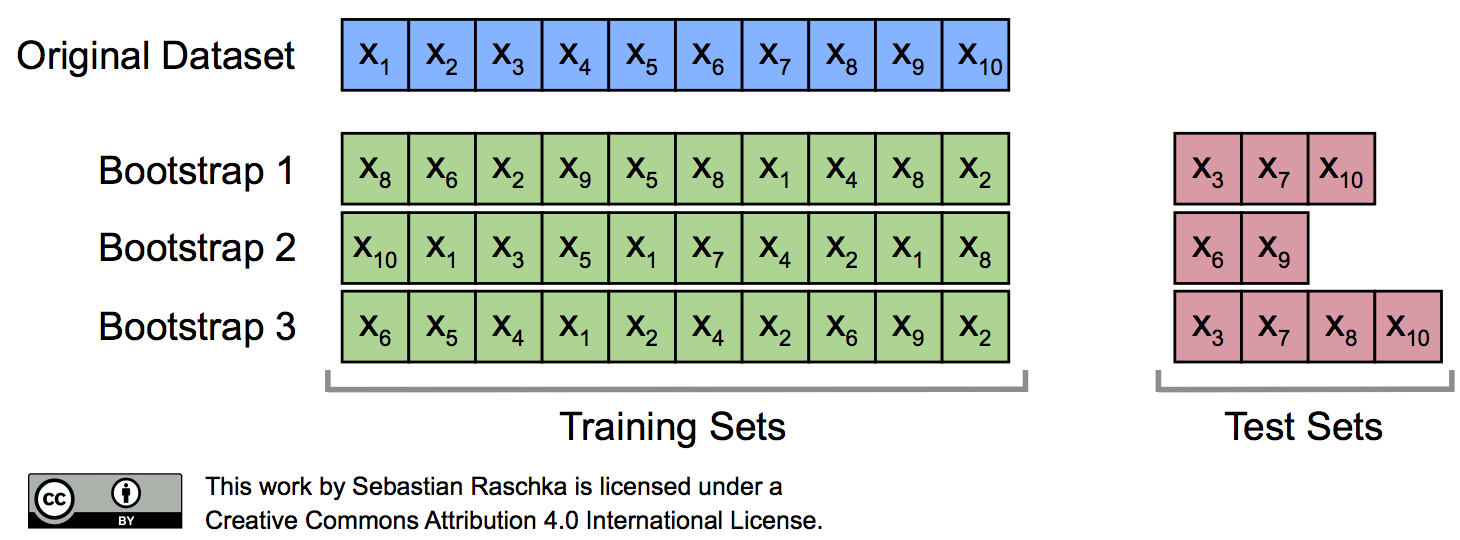
\includegraphics[width=0.7\textwidth]{figure_man/bootrap_concept.png}
% \end{center}
  \item From the resulting $B$ test errors, we can, for instance, use the 2.5~\%-quantile $q_{0.025}$ and the 97.5~\%-quantile $q_{0.975}$ to estimate a 95~\%-CI:
$\left[q_{0.025}, q_{0.975}\right].$
\end{itemize}

\end{vbframe}


%
% \begin{vbframe}{Train vs. test error}
%
% <<overfitting-polynomial-prep, echo=FALSE, out.width="0.9\\textwidth", fig.height=5>>=
% .h = function(x) 0.5 + 0.4 * sin(2 * pi * x)
% h = function(x) .h(x) + rnorm(length(x), mean = 0, sd = 0.05)
%
%  set.seed(1234)
% x.all = seq(0, 1, length = 21L)
% ind = seq(1, length(x.all), by = 2)
%
%  x = x.all[ind]
% y = h(x)
% x.test = x.all[-ind]
% y.test = h(x.all[-ind])
%
%  line.palette = pal_3
% baseplot = function() {
%   par(mar = c(2, 2, 1, 1))
%   plot(.h, lty = 2L, xlim = c(0, 1), ylim = c(-0.1, 1), ylab = "y, f(x)", xlab = "")
%   points(x, y, pch = 19L)
%   points(x.test, y.test)
%   legend(x = "bottomleft", inset= 0.1, legend = c("true relationship f(x)", "training set", "test set"),
%     col = "black", lty = c(2L, NA, NA), pch = c(NA, 19L, 21L))
% }
%
%  mods = list(
%   p1 = lm(y ~ poly(x, 1, raw = TRUE)),
%   p2 = lm(y ~ poly(x, 5, raw = TRUE)),
%   p4 = lm(y ~ poly(x, 11, raw = TRUE)))
% x.plot = seq(0, 1, length = 500L)
% baseplot()
% @
% <<overfitting-polynomial-plot, echo=FALSE, out.width="0.9\\textwidth", fig.height=2.7>>=
% baseplot()
% for (i in seq_along(mods)) {
%   lines(x.plot, predict(mods[[i]], newdata = data.frame(x = x.plot)),
%     col = line.palette[i], lwd = 2L)
% }
% legend("topright", paste(sprintf("d = %s", c(1, 5, 11)), c("(underfit)", "(good)", "(overfit)")),
%   col = line.palette, lwd = 2L)
% @
% \lz
% Train and test error:
% <<polynomial-train-test-plot, echo=FALSE, out.width="0.9\\textwidth", fig.height=2.7>>=
% d = lapply(1:11, function(i) {
%   mod = lm(y ~ poly(x, degree = i, raw = TRUE))
%   list(
%     train = mean((y - predict(mod, data.frame(x = x)))^2),
%     test = mean((y.test - predict(mod, data.frame(x = x.test)))^2)
%   )
% })
% par(mar = c(4, 4, 1, 1))
% #par(mar = c(4, 4, 0, 0) + 0.1)
% plot(1, type = "n", xlim = c(1, 11), ylim = c(0, 0.05),
%   ylab = "MSE", xlab = "degree of polynomial")
% lines(1:11, sapply(d, function(x) x$train), type = "b", lwd = 3, lty = 2)
% lines(1:11, sapply(d, function(x) x$test), type = "b", col = "gray", lwd = 3, lty = 1)
%
%  legend("top", c("training error", "test error"), lty = c(2,1), col = c("black", "gray"), lwd = 3)
% text(3.75, 0.02, "High Bias,\nLow Variance", bg = "white")
% arrows(4.75, 0.02, 2.75, 0.02, code = 2L, lty = 2L, length = 0.1)
%
%  text(8, 0.02, "Low Bias,\nHigh Variance", bg = "white")
% arrows(9, 0.02, 7, 0.02, code = 1, lty = 2, length = 0.1)
% @
%
% \end{vbframe}


\begin{vbframe}{Resampling Methods}

\begin{itemize}
  \item Aim: Assess the performance of an \textbf{algorithm} (not just a model).
  \item Resampling methods use the available data more efficiently than a simple train-test split.
  \item The data is split repeatedly into training and test sets. Later, we aggregate (e.g., average) the results.
  \item The usual trick is to make training sets quite large (to keep the pessimistic bias small),
  and to handle the variance introduced by smaller test sets through many repetitions and averaging
  of results.
\end{itemize}

\begin{center}
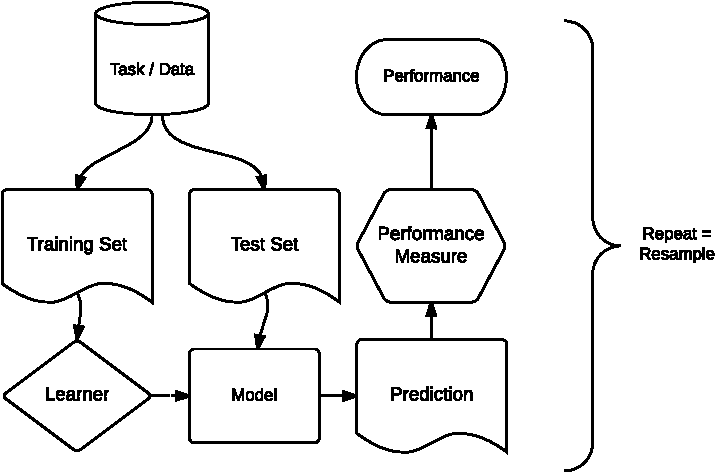
\includegraphics[width=5cm]{figure_man/ml_abstraction-crop.pdf}
\end{center}

\end{vbframe}


\begin{vbframe}{Generalization Error of Learning Algorithms}

A learning algorithm (inducer) $\mathcal{I}_{L, O}(\Dtrain)$ that is applied to training data $\Dtrain$, consisting of $n$ randomly drawn observations from $\Pxy$, produces a prediction model $\fh_{\Dtrain}(\xv) = \mathcal{I}_{L, O}(\Dtrain)$.

\lz

The \textbf{generalization error of a learning algorithm} $\mathcal{I}_{L, O}$ is the expectation of the generalization error of $\fh_{\Dtrain}$ w.r.t. all possible training sets $\Dtrain$ of size $n$ that were drawn from $\Pxy$:
\begin{eqnarray*}
\GEind &=& \E_{\Dtrain \sim \Pxy}\left(GE(\fh_{\Dtrain})\right) \\
&=& \E_{\Dtrain \sim \Pxy}\left( \E_{\xy \sim \Pxy}( L(y, \fh_{\Dtrain}(\xv)) | \Dtrain) \right).
\end{eqnarray*}
%&=& \frac{1}{B} \sum_{b = 1}^{B} \widehat{GE}(\fh_{\Dtrain^b}, \Dtest^b)\\
%&=& \frac{1}{B} \sum_{b = 1}^{B} \frac{1}{|\Dtest^b|} \sum_{\xyi \in \Dtest^b} L(\yi, \fh_{\Dtrain^b}(\xi))
%Note that the expectation $\EDn$ averages over the randomness caused by drawing the data sets $\D$ of size $n$ used to produce $\fh_{\D}$.
%averages over everything that is random, including the randomness in the data $\D$ that produced $\fh_{\D}$.

\lz

$\Rightarrow$ Resampling methods estimate this so-called \textbf{expected generalization error} which is a property of the inducing algorithm $\mathcal{I}_{L, O}$ (i.e., \textbf{not} of a specific model $\fh_{\D}$).

\framebreak

Resampling methods are based on repeatedly splitting the observed dataset into training and test sets and fitting a learning algorithm to training sets of equal size $n$.

\lz

Consider $B$ sets of training and test data generated by a resampling method (denoted by $\Dtrain^b$ and $\Dtest^b$, $b=1,\dots,B$, respectively). The \textbf{expected generalization error} can then be estimated by
\begin{eqnarray*}
\widehat{\GEind} &=&
\frac{1}{B} \sum_{b = 1}^{B} \GEh{\Dtest^b} (\fh_{\Dtrain^b})\\
&=& \frac{1}{B} \sum_{b = 1}^{B} \frac{1}{|\Dtest^b|} \sum_{\xy \in \Dtest^b} L\left(y, \fh_{\Dtrain^b}(\xv)\right).
\end{eqnarray*}
\textbf{Note}: $\GEind$ depends on $n$, i.e., the size of the training sets.

\end{vbframe}

\endlecture
\end{document}

